\section{Anhang: Die Originalmessdaten}
\label{sec:anhang}

\begin{figure}
    \centering
    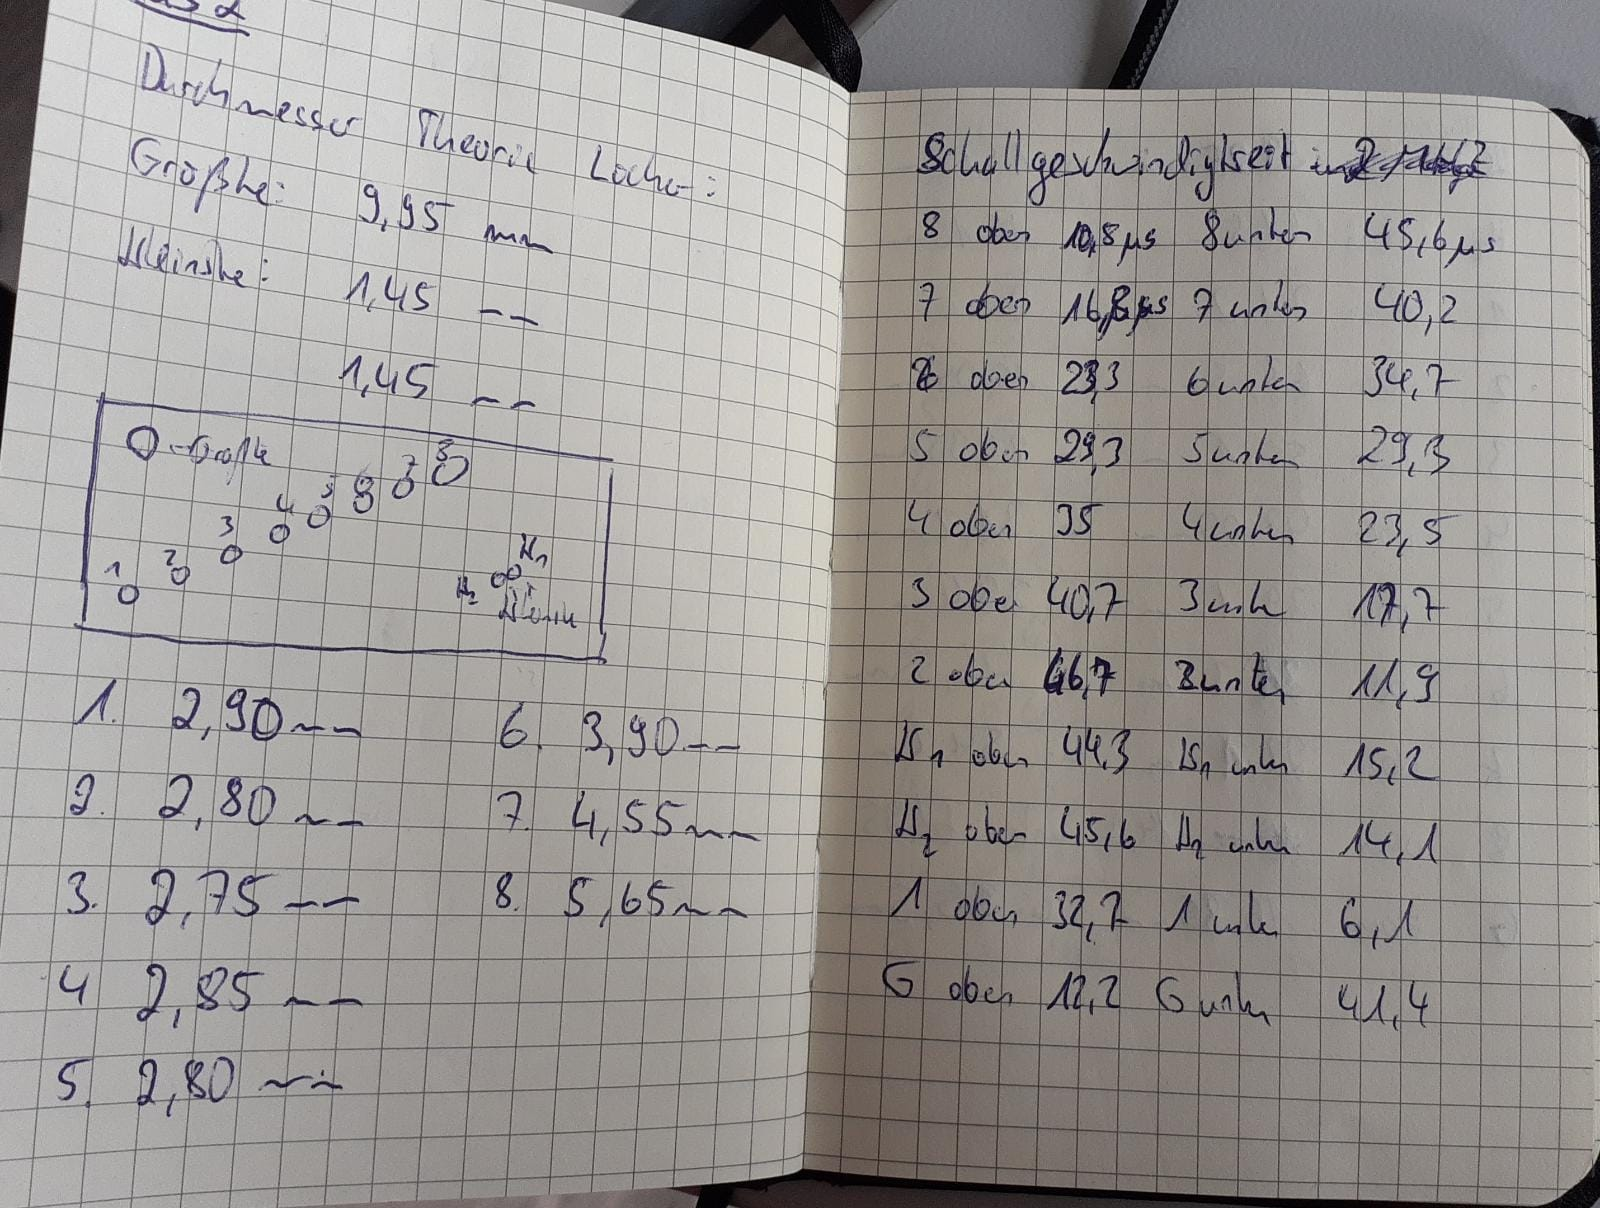
\includegraphics[width = 7cm]{content/mess1}
    \caption{Die gemessenen Werte.}
    \label{fig:mess1}
\end{figure}


\begin{figure}
    \centering
    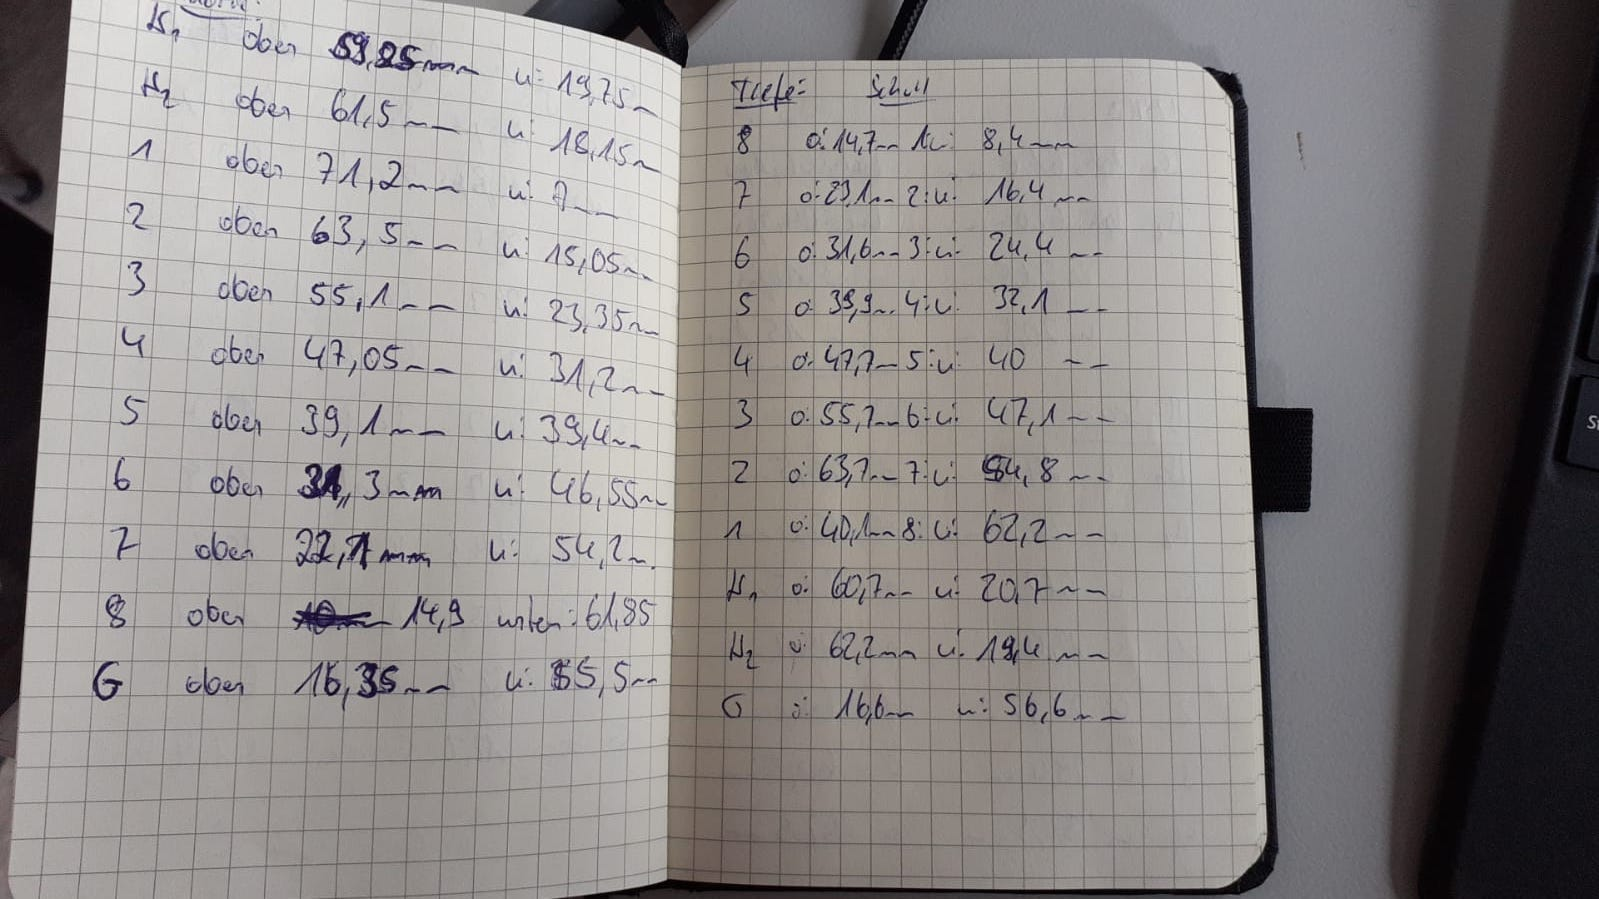
\includegraphics[width = 7cm]{content/mess2}
    \caption{Die gemessenen Werte.}
    \label{fig:mess2}
\end{figure}


\begin{figure}
    \centering
    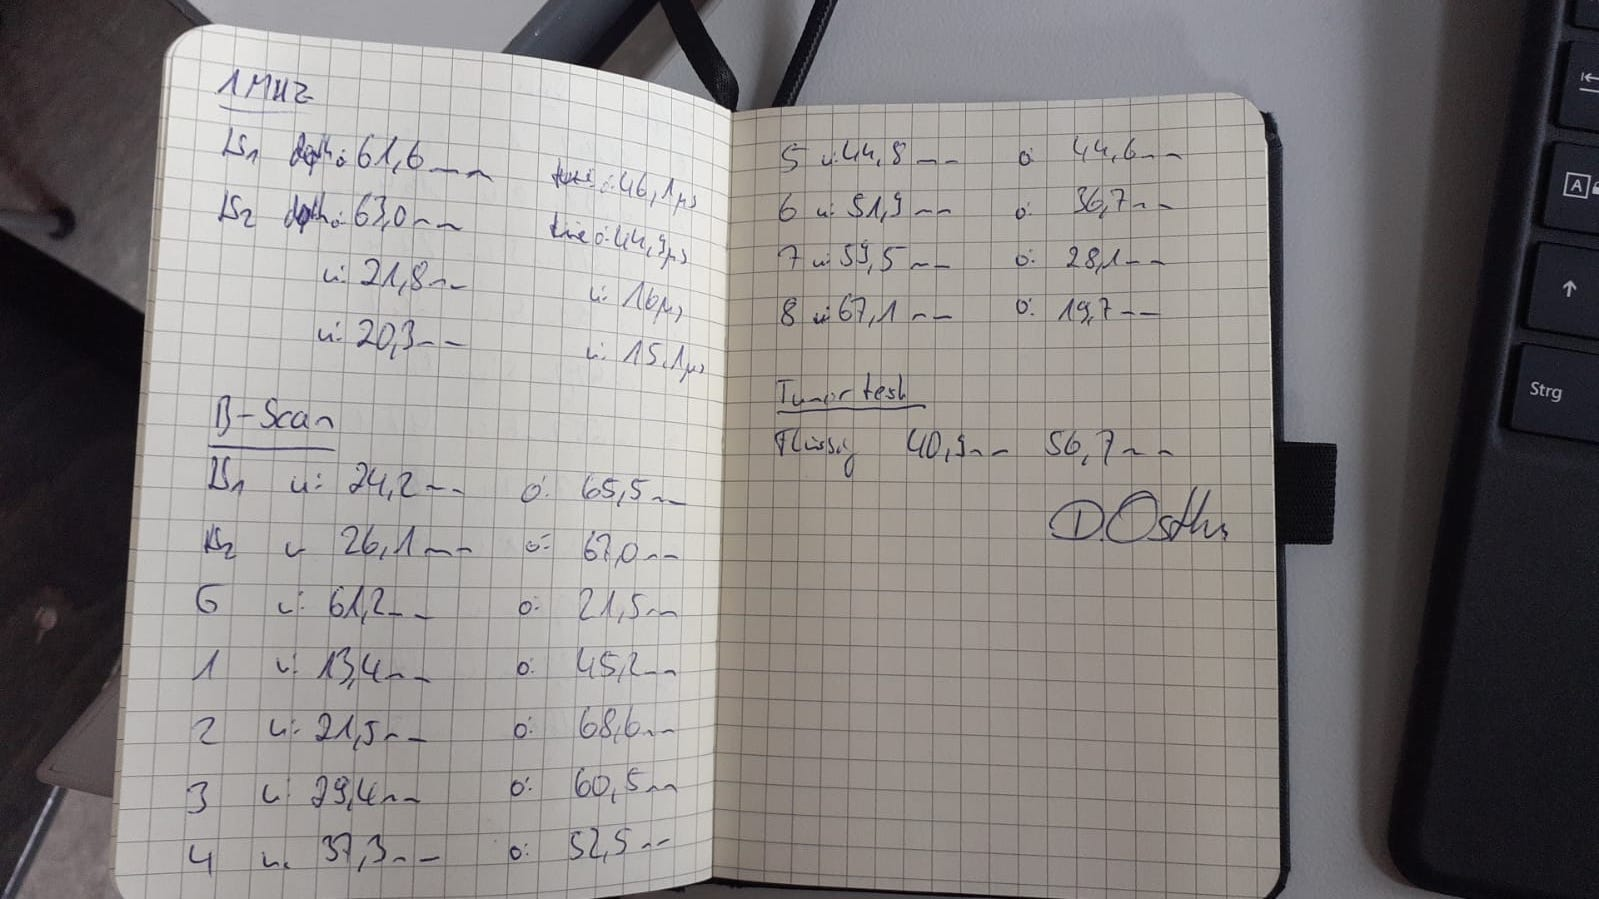
\includegraphics[width = 7cm]{content/mess3}
    \caption{Die gemessenen Werte.}
    \label{fig:mess3}
\end{figure}
